% Chapter Template

\chapter{Software Framework} % Main chapter title

\label{Chapter4} % Change X to a consecutive number; for referencing this chapter elsewhere, use \ref{ChapterX}

\lhead{Chapter 4. \emph{Software Framework}} 
		The ROS\cite{quigley2009ros} is the de facto standard used for any robotics related research in the recent times. However it is officially supported only for the Ubuntu distribution which makes it unavailable to the people who work with sensors that are being support only for Windows system (i.e Kinect for windows v2). Hence a distributed architecture which is not specific to any operating system or programming language is proposed which uses open network communication standards and transparent message passing using structured data. In this chapter the design philosophy of the software framework and core components of the system are explained.
		
\section{Framework Design}		
	The system could contain nodes/processes which can be running in the same computer or might be running anywhere in the network. The order of start and stop of these nodes essentially do not matter.
\subsection{Communication Protocol}	
	The nodes communicate with each other as shown in Fig~\ref{fig:framework} using either inproc/IPC/TCP/UDP protocols depending on its location and to whom it wants to communicate with. The communication between the nodes is established using ZeroMQ\cite{ZeroMQ} library which has a variety of advantages any modern application would require like  
\begin{itemize}
\item Multiple language and Cross platform
\item Message using inproc, IPC, TCP, UDP protocols
\item Support for patterns like Publisher-Subscriber, Push-Pull, Request-Response
\item Tiny and high-speed asynchronous implementation
\end{itemize}
	ZeroMQ comes with the low-level C API. High-level bindings exist in 40+ languages including Python, Java, PHP, Ruby, C, C++, C\#, Erlang, Perl, and more. So it can run in literally any OS and owing to its very low memory foot print it can also run on the mobile devices and tablets.
\begin{figure}
\centering
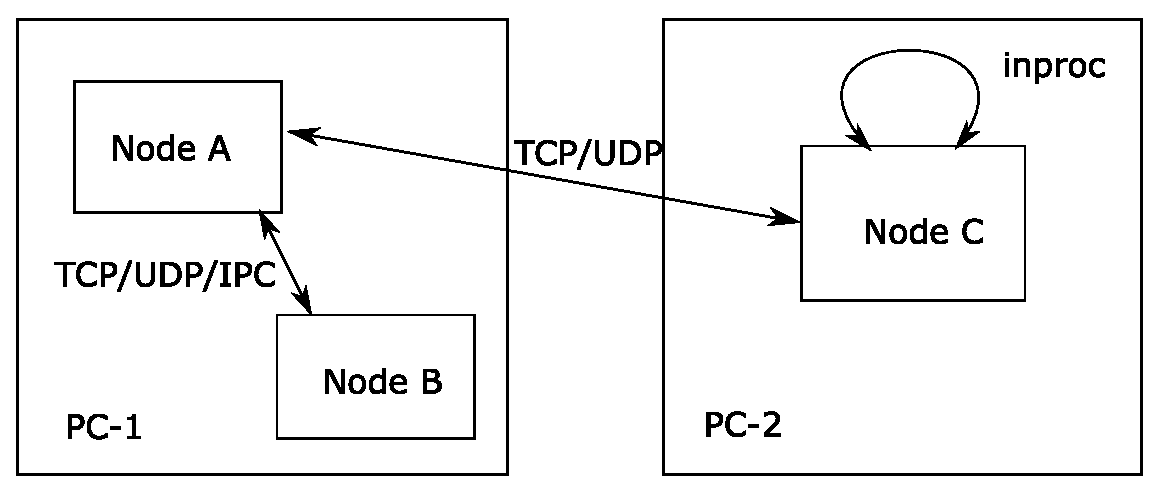
\includegraphics[width=\textwidth]{assets/architecture_comm.eps}
\caption[Framework Communication Protocol]{Framework Communication Protocol}
\label{fig:framework}
\end{figure}
\subsection{Message Format}
	The nodes communicate with each other using structured data formatted using the Google Protocol buffers\cite{ProtocolBuffers}. Protocol buffers are Google's language-neutral, platform-neutral, extensible mechanism for serializing structured data. It could be thought of as XML format, but smaller, faster, and simpler. The data could be structured once as per the requirement, then the special generated source code could be integrated with the application to easily write and read structured data to and from a variety of data streams and using a variety of languages – Java, C++, C\# or Python. The message is defined in a file with extension *.proto which will be consumed by the code generator to generate code for a specific language. A sample proto file is shown in Fig~\ref{fig:protobuf_def} and the code generation principle is shown in Fig~\ref{fig:protobuf_codegen}
\begin{figure}
\centering
\begin{subfigure}[t]{0.48\textwidth}
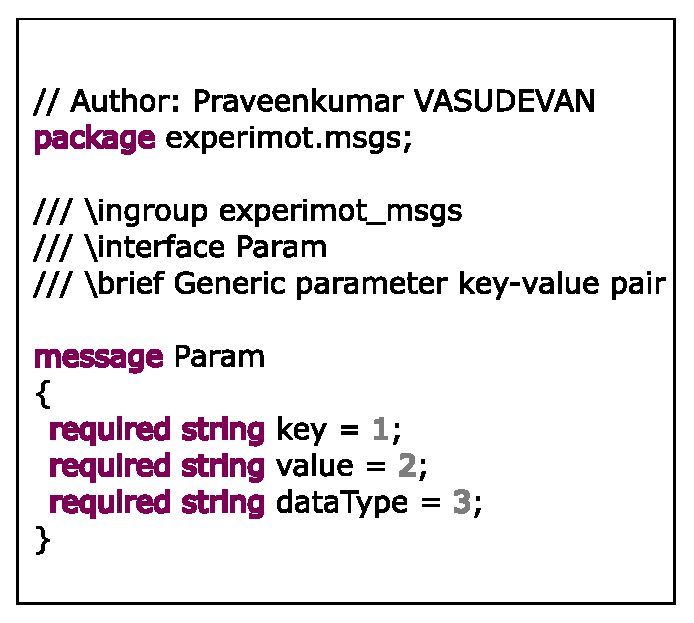
\includegraphics[width=\textwidth]{assets/protobuf_definition.eps}
\caption[Message Definition]{Message Definition}
\label{fig:protobuf_def}
\end{subfigure}
\begin{subfigure}[t]{0.48\textwidth}
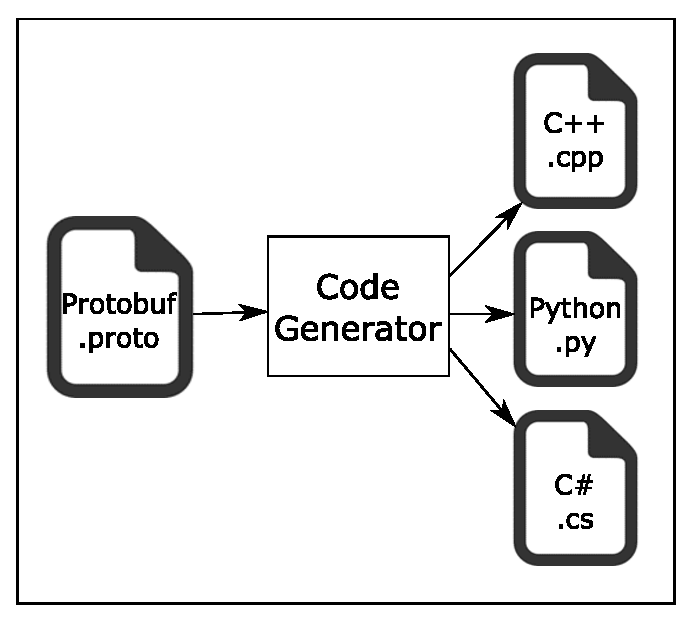
\includegraphics[width=\textwidth]{assets/protobuf_codegen.eps}
\caption[Code Generation]{Code Generation}
\label{fig:protobuf_codegen}
\end{subfigure}
\caption[Google Protocol Buffers]{Google Protocol Buffers}
\label{fig:protobuf}
\end{figure}
\subsection{Configuration File}
	An XML configuration file to manage the nodes and system/node level parameters is proposed. The format of the XML file is designed using an XML schema definition (XSD) language. The schema representation is shown in the Fig~\ref{fig:config_xsd}. The important strongly typed components of the schema are
	\begin{itemize}
	\item Parameters: These are the global parameters composed of key, value and the type of the parameter. The supported types are boolean, integer, double, string and comma separated values(CSV). 
	\item Nodes: These are the individual processes that would compose an application as a whole. Each of these nodes could be written in any programming language supported by the communication protocol and message serialization library. Each node in turn is composed of
	\begin{itemize}
	\item Name : A name unique to this node
	\item Enable/Disable Flag: A flag to tell the application if this node has to be started when the application starts up.
	\item Type: The type is the user-defined role of the node.
	\item Process Information: The executable/script along with a set of arguments associated with this node.
	\item Parameters: These are the node level parameters with the structure similar to the global parameters. A node level parameter can override the global parameter with the same name.
	\item Publishers: A set of publisher which publishes a message (structured using proto format) on a specific topic over a configured communication channel (TCP/UDP/IPC etc.,). Usually the publishers relates to the data produced by this node.
	\item Subscribers: A set of subscriber which listens to a message of specific type publish on a specific topic over a specific communication channel. The subscribers relates to the data consumed by this node.
	\end{itemize}
	\end{itemize}
\begin{figure}
\centering
%\begin{subfigure}[t]{0.48\textwidth}
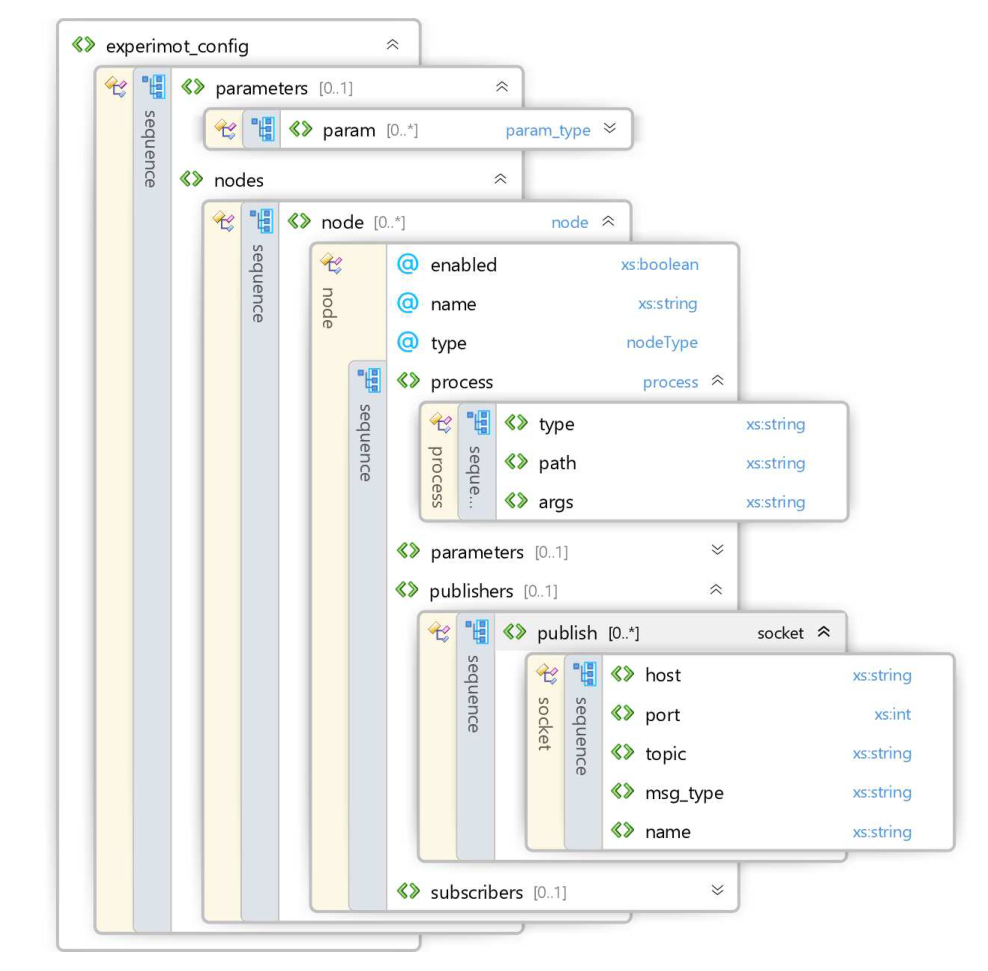
\includegraphics[width=\textwidth]{assets/xsd_config.eps}
\caption[Configuration XML Schema Definition]{Configuration XML Schema Definition}
\label{fig:config_xsd}
%\end{subfigure}
%\begin{subfigure}[t]{0.48\textwidth}
%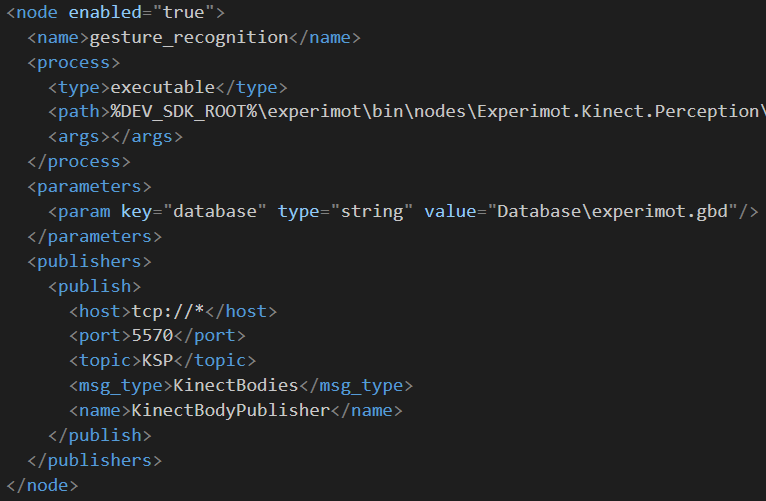
\includegraphics[width=\textwidth]{assets/xml_config_sample.png}
%\caption[Code Generation]{Code Generation}
%\label{fig:protobuf_codegen}
%\end{subfigure}
%\caption[Google Protocol Buffers]{Google Protocol Buffers}
%\label{fig:protobuf}
\end{figure}
\subsection{An example usage of the framework}
In order to demonstrate how the framework described so far could be used for developing a distributed application, a sample application scenario is considered. A \emph{robot\_interace\_node} node reads the joint values of the robot and publishes them over a topic \textbf{RJV} (robot joint values). Another node namely \emph{visualization\_node} subscribes to the topic \textbf{RJV} and each time it receives the new joint values updates the robot joint position being shown by the visualization engine. The pseudo-code of these nodes are shown in Fig~\ref{fig:node_a} and Fig~\ref{fig:node_b} respectively.
\begin{figure}[H]
%\centering
\begin{subfigure}[t]{0.48\textwidth}
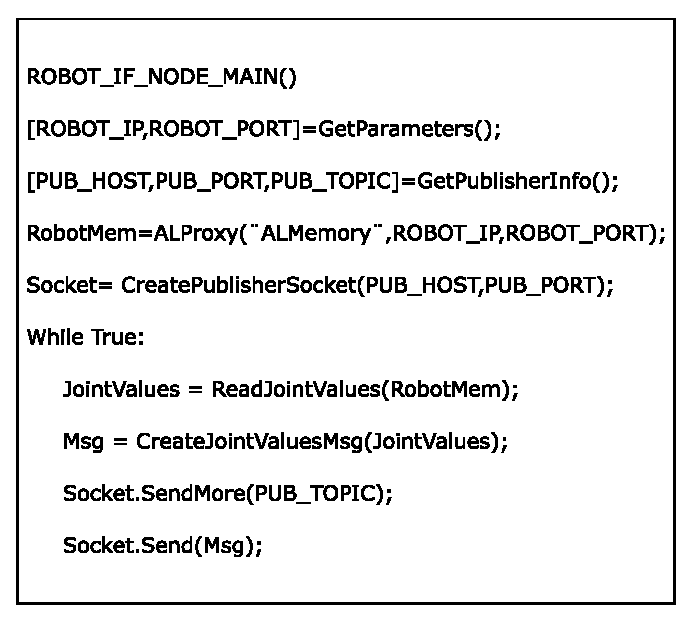
\includegraphics[width=\textwidth]{assets/sample_node_A.eps}
\caption[Robot Interface Node]{Robot Interface Node}
\label{fig:node_a}
\end{subfigure}
\begin{subfigure}[t]{0.48\textwidth}
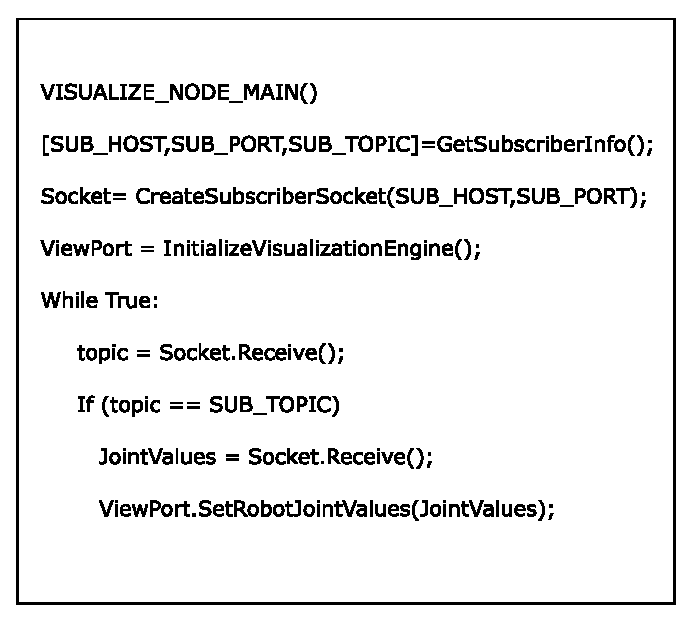
\includegraphics[width=\textwidth]{assets/sample_node_B.eps}
\caption[Visualization Node]{Visualization Node}
\label{fig:node_b}
\end{subfigure}
\caption[Sample nodes]{Sample nodes}
\label{fig:pseudo_nodes}
\end{figure}
And finally we can define a configuration file which contains the parameters and start up information needed by the application to start up these node. A sample configuration file for this scenario is shown in Listing~\ref{lst:sample_config}

\lstinputlisting[caption=Sample XML Configuration File,label={lst:sample_config},language=XML]{assets/sample_config.xml}
